% Copyright (c) 2026 Roger Román Armoa García
% SPDX-License-Identifier: CC-BY-NC-SA-4.0

\documentclass[12pt,a4paper]{article}

% -------------------------------------------------
% Paquetes
% -------------------------------------------------
\usepackage[spanish,es-nodecimaldot]{babel}
\usepackage[utf8]{inputenc}
\usepackage[T1]{fontenc}
\usepackage{lmodern}
\usepackage{siunitx}
\usepackage{amssymb}
\usepackage{csquotes}
\usepackage{float}
\usepackage{colortbl}
\usepackage{booktabs}
\usepackage{tabularx}
\usepackage{placeins}
\usepackage[a4paper,margin=2.5cm]{geometry}
\usepackage{setspace}
\usepackage{amsmath}
\usepackage{graphicx}
\usepackage{pdfpages}
\usepackage{microtype}
\usepackage{xcolor}
\usepackage{titlesec}
\usepackage[hidelinks]{hyperref}
\usepackage[backend=biber,style=apa,sorting=nyt]{biblatex}
\usepackage[most]{tcolorbox}
\usepackage{pifont}
\usepackage{pdflscape}
\usepackage{longtable}

\addbibresource{referencias.bib}

% -------------------------------------------------
% Colores
% -------------------------------------------------
\definecolor{calAzul}{RGB}{30,80,125}
\definecolor{calAzulClaro}{RGB}{215,230,245}
\definecolor{calVerdeClaro}{RGB}{225,240,225}
\definecolor{calAmarilloClaro}{RGB}{250,240,200}
\definecolor{calGrisClaro}{RGB}{235,235,235}

% -------------------------------------------------
% Formato de títulos
% -------------------------------------------------
\titleformat{\section}
  {\normalfont\Large\bfseries}
  {\thesection}{1em}{}

\titleformat{\subsection}
  {\normalfont\large\bfseries}
  {\thesubsection}{1em}{}

\titleformat{\subsubsection}
  {\normalfont\normalsize\bfseries}
  {\thesubsubsection}{1em}{}

% -------------------------------------------------
% Inicio
% -------------------------------------------------
\begin{document}

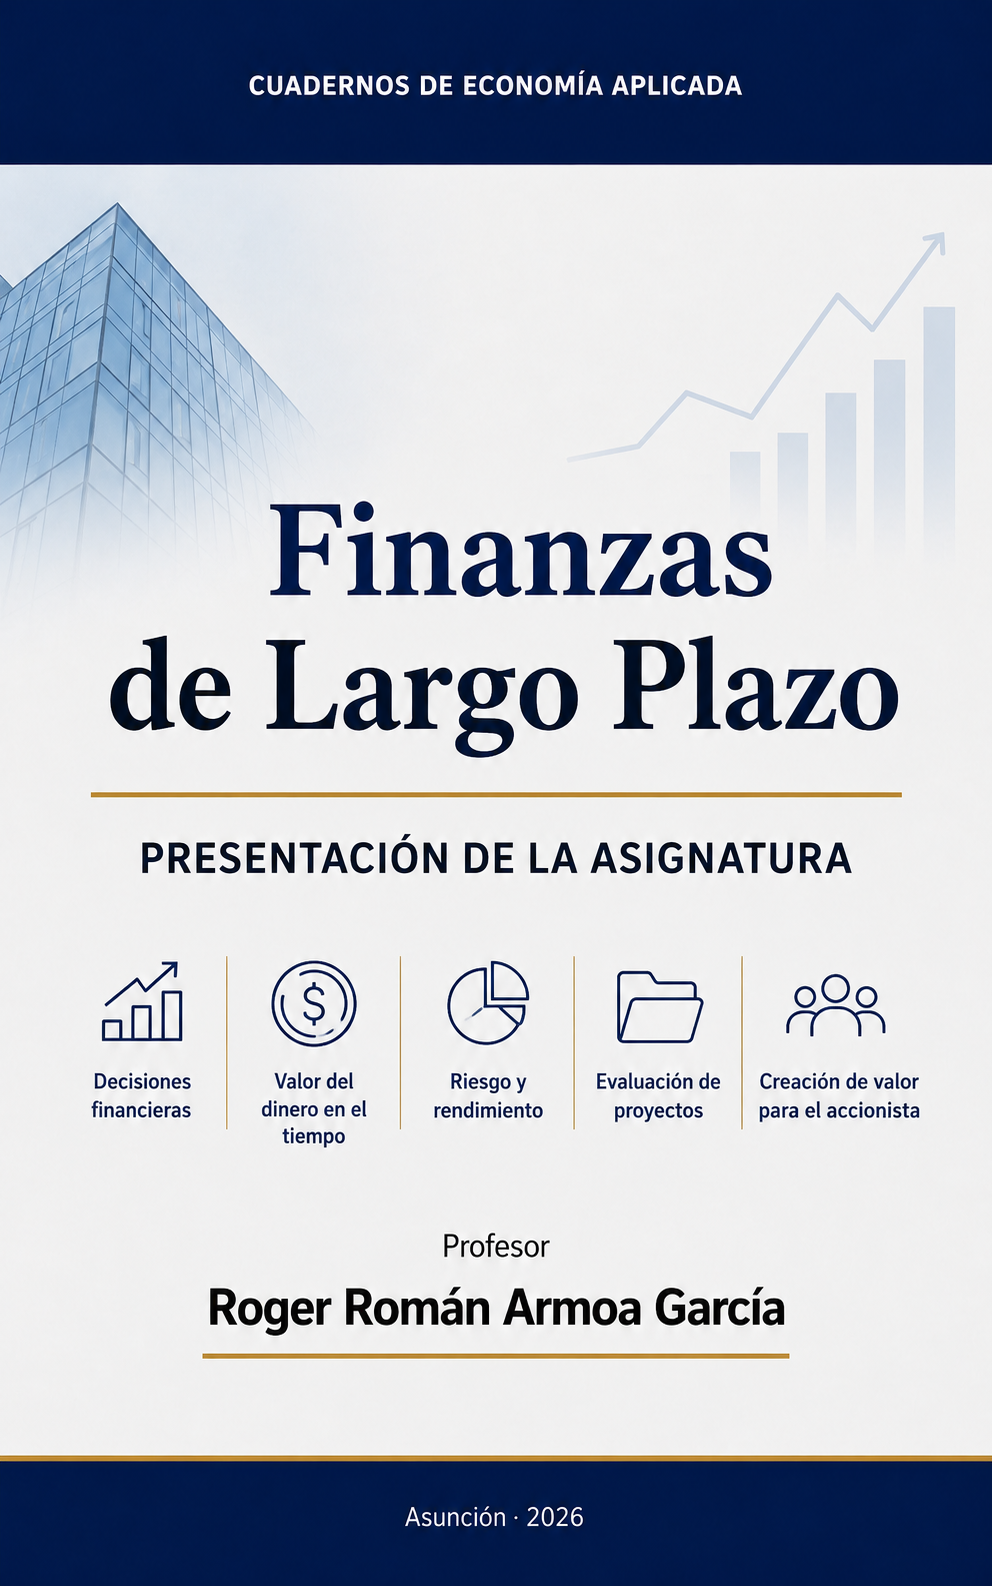
\includepdf[pages=1,fitpaper=true]{portada_presentacion_asignatura_v1.png}

\thispagestyle{empty}
\begin{center}
\Large\textbf{Finanzas Largo Plazo 2026}\\[0.3cm]
\large\textbf{Volumen 6}\\[0.3cm]
\large Roger Román Armoa García\\[0.2cm]
\normalsize Asunción -- 2026
\end{center}

\vfill

\begin{center}
\textbf{Colección}\\[0.15cm]
\textit{Cuadernos de Finanzas Largo Plazo}\\[0.3cm]
Universidad Americana\\
Campus Asunción\\
Facultad Ciencias Económicas y Administrativas\\
Materia homóloga\\[0.3cm]
Editor académico: Roger Román Armoa García
\end{center}

\vfill

\noindent
Esta colección simplifica el estudio de la asignatura en Modelo de Aprendizaje Basado en Competencias (MAC).\parencite{uaModeloCompetencias}

\newpage

\section*{Página legal}

\textbf{Finanzas Largo Plazo 2026}\\
Colección: Cuadernos de Finanzas Largo Plazo\\
Volumen 6\\[0.2cm]

\textbf{Autor:}\\
Roger Román Armoa García\\[0.2cm]

\textbf{Filiación Institucional:}\\
Universidad Americana\\[0.2cm]

\textbf{Carácter de la Materia:}\\
Asignatura homóloga / transversal\\[0.2cm]

Asignatura: Finanzas Largo Plazo\\
Código de la asignatura: ICA-035\\[0.2cm]

Asunción, Paraguay\\
Primera edición: 2026\\[0.2cm]

© 2026 Roger Román Armoa García\\[0.2cm]

Clasificación Decimal Dewey: 658.15\\
ISBN:pendiente de asignacion

\newpage

\tableofcontents
\newpage

\begin{tcolorbox}[
colback=gray!5,
colframe=black,
title=\textbf{Datos de identificación del trabajo},
sharp corners,
boxrule=0.8pt,
width=\textwidth
]

\renewcommand{\arraystretch}{1.8}

\begin{tabular}{p{0.24\textwidth} p{0.70\textwidth}}

\textbf{Nombre y apellido:} & \hrulefill \\

\textbf{Asignatura:} &
Finanzas a Largo Plazo \\

\textbf{Carrera:} &
Economía \\

\textbf{Facultad:} &
Facultad de Ciencias Económicas y Administrativas \\

\textbf{Universidad:} &
Universidad Americana \\

\textbf{Grupo/Sección:} &
Grupo 80 -- Presencial \\

\textbf{Docente:} &
Roger Román Armoa García \\

\textbf{Fecha:} &
\hrulefill \\

\end{tabular}

\end{tcolorbox}

\section{Introducción a la modalidad de enseñanza por competencias}

\subsection{Enfoque general de la asignatura}

En esta modalidad de enseñanza el profesor asume el papel de guía del aprendizaje y es el alumno quien construye los conocimientos y muestra evidencias de que adquiere la competencia. Por esta razón, uno de los primeros puntos que definimos con los alumnos es la competencia que queremos lograr en la asignatura, luego en la unidad y, por último, en la clase.\parencite{uaModeloCompetencias,armoa2026planeamiento}

\subsection{Evidencias de aprendizaje}

Mi propuesta para que muestren evidencias de que adquieren la competencia que buscamos consiste en la elaboración y presentación de un PDF. Por esta razón, una de las primeras asignaciones consiste en que cada uno elabore informes en formato PDF con la herramienta de software que prefiera.

El profesor realiza correcciones sucesivas sobre este trabajo hasta llegar al formato que queremos obtener en el documento final.

De manera general, el proceso consiste en:

\begin{itemize}
\item elaborar una primera versión del PDF;
\item presentar el trabajo para su revisión;
\item recibir observaciones y correcciones;
\item realizar los ajustes necesarios;
\item presentar nuevas versiones hasta alcanzar el formato esperado.
\end{itemize}

\begin{figure}[H]
    \centering
    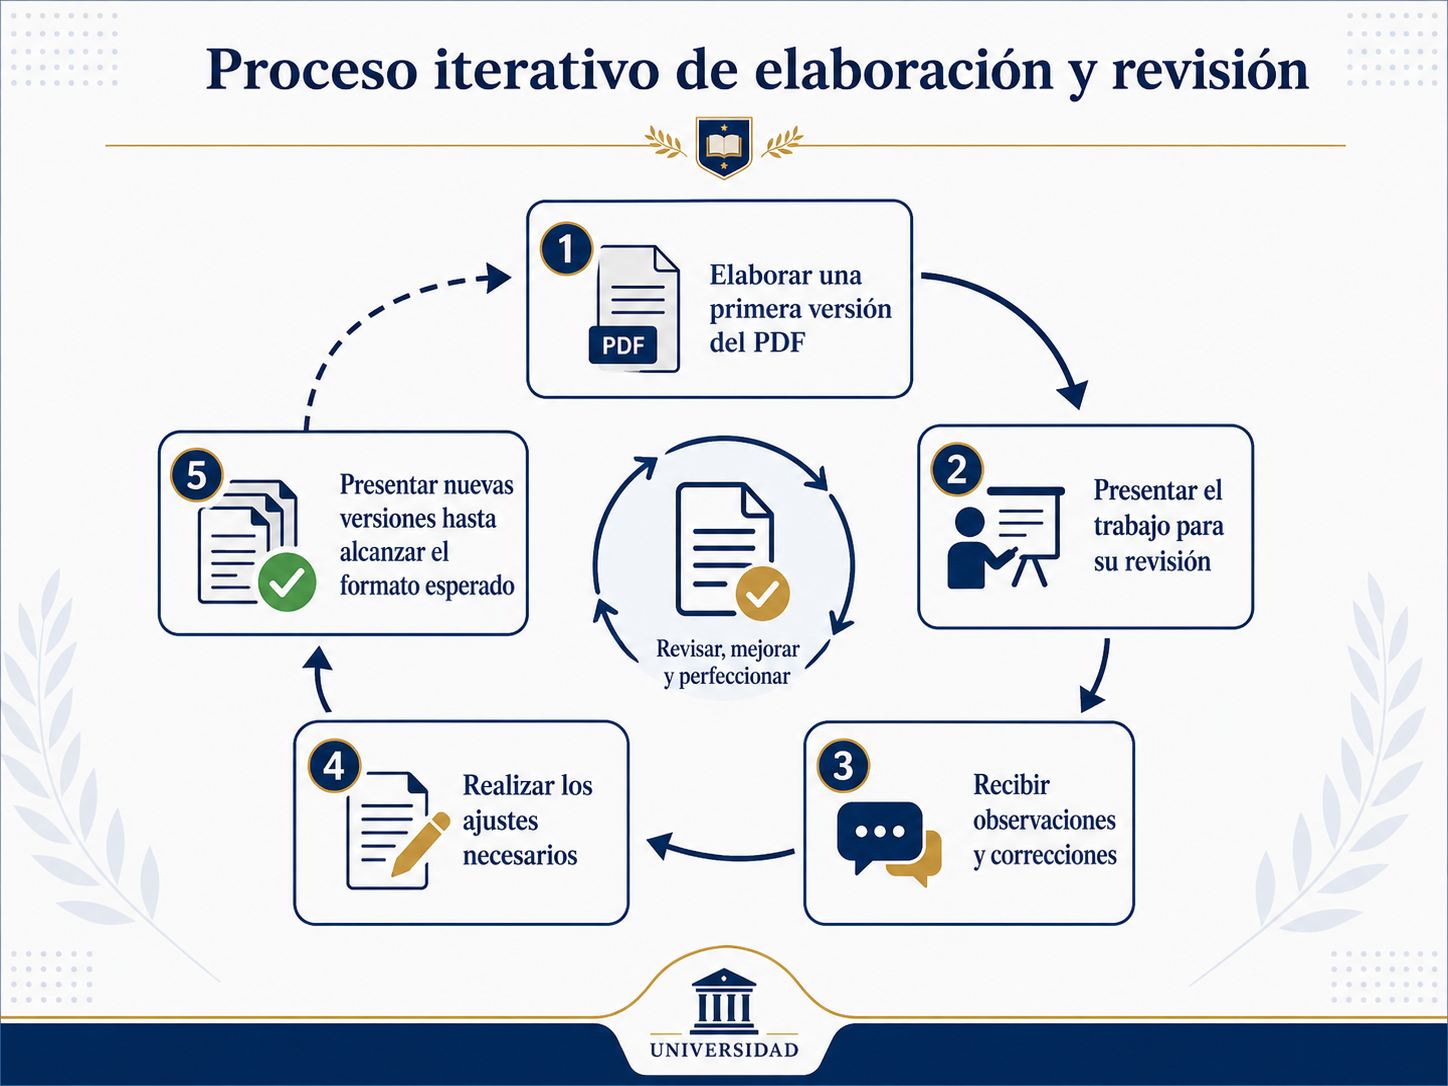
\includegraphics[width=0.50\textwidth]{proceso_iterativo.png}
    \caption{Proceso iterativo de elaboración y revisión del material.}
    \label{fig:proceso_iterativo}
\end{figure}

\subsection{Presentación e integración del grupo}

También me interesa conocerlos personalmente, ya que nuestra modalidad es presencial. Por eso, les pido que completen el formulario de datos personales y que se acerquen a mí para conversar brevemente.

También podemos realizar una presentación ante todo el grupo. El objetivo es que yo los conozca y que ustedes se conozcan entre sí. Es una actividad para romper el hielo que parece trivial, pero es importante porque esta es una asignatura homóloga, es decir, participan alumnos de distintas carreras.

\subsection{Propósito de la primera actividad}

No los subestimo al pedirles que preparen un PDF. Es muy probable que ustedes ya manejen estas herramientas mejor que estudiantes de promociones anteriores, por así decirlo. Sin embargo, con frecuencia encuentro dificultades que son muy comunes al elaborar un informe, y me interesa que nos preparemos bien en este aspecto para evitar esos mismos problemas.

\subsection{Clases en Aula}

Por su carácter aplicado, la asignatura contempla actividades prácticas en aula. Para estas actividades se utilizan recursos informáticos asignados institucionalmente, de acuerdo con su disponibilidad y con la planificación correspondiente a cada clase.\parencite{armoa2026planeamiento}

En las aulas no contamos con ordenadores, pero si contamos con WIFI, además de recursos para presentación y conectividad para el profesor. Cuando el acceso a los equipos requiere credenciales, estas son proporcionadas conforme a los procedimientos definidos por los responsables de la sala.

Las actividades de laboratorio se articulan con la metodología de construcción de clases adoptada en la asignatura. El docente presenta una orientación inicial y los estudiantes desarrollan las tareas prácticas, recopilan y contrastan información, construyen evidencias de aprendizaje y aportan los resultados obtenidos a la base de conocimientos que se discute y valida durante la clase.

Para facilitar la coordinación previa y posterior a los encuentros presenciales, se utiliza un canal de mensajería instantánea definido para el grupo. Durante el periodo académico 2026 se propone el uso de WhatsApp como medio complementario de comunicación para informar el lugar de inicio de la clase, los laboratorios asignados y otras cuestiones operativas relacionadas con el desarrollo de las actividades.

Este canal complementa, pero no sustituye, los medios académicos e institucionales que correspondan. Su utilización facilita especialmente la coordinación de las actividades que se desarrollan fuera del aula o del laboratorio, dado que la carga académica de la asignatura incluye tanto trabajo con acompañamiento docente como trabajo independiente.

\subsection{Medición de la competencia adquirida}

La adquisición de competencias requiere un proceso de medición que permita comparar los resultados alcanzados con la situación inicial de los estudiantes. Esta medición se considera en tres niveles: asignatura, unidad didáctica y clase.

Por razones de practicidad, en esta primera experiencia proponemos realizar una medición diagnóstica y formativa inicial a nivel general de la asignatura. Su propósito es disponer de un punto de referencia que permita reconocer los conocimientos y competencias que los estudiantes poseen al comienzo del periodo académico y, posteriormente, contrastarlos con los resultados que alcanzan durante el desarrollo de la asignatura.\parencite{armoa2026planeamiento}

Además de identificar el nivel inicial de competencias, resulta importante conocer los intereses académicos y profesionales de los estudiantes. Por esta razón, el instrumento inicial incluye información sobre la carrera de procedencia y sobre las áreas de interés de cada participante. La lectura de estas respuestas permite obtener, desde la primera clase, una aproximación al nivel de conocimientos del grupo y a sus principales ámbitos de interés.

Esta información contribuye a orientar las actividades de aprendizaje y a evitar, en la medida de lo posible, una dedicación innecesaria de tiempo a contenidos que el grupo ya domina. El tiempo disponible para la asignatura constituye un recurso limitado y, por ello, se procura destinarlo prioritariamente a actividades que aporten valor al aprendizaje y que resulten útiles a corto, mediano y largo plazo.

La medición inicial se integra con la metodología de construcción de clases adoptada en la asignatura. A partir del diagnóstico, el docente presenta una estructura inicial de temas y subtemas, mientras que los estudiantes construyen y amplían la base de conocimientos, incorporan información a la matriz de trabajo y participan en la discusión y validación de los contenidos desarrollados.

\subsubsection{Registro de asistencia}

La asignatura requiere también un registro sistemático de la asistencia presencial. Debido a que este grupo aplica este requisito de manera especialmente rigurosa, se establece inicialmente un procedimiento operativo que puede ser revisado y perfeccionado a medida que se evalúa su funcionamiento.

\subsection{Medios digitales}

Para el registro de las evidencias de participación que habitualmente se consignan mediante la firma del docente en el cuaderno, los estudiantes pueden utilizar también dispositivos digitales, como tabletas.

Cuando el dispositivo dispone de un lápiz digital que permite incorporar escritura manuscrita, el docente puede realizar la firma directamente sobre el documento o archivo correspondiente. En estos casos, el estudiante es responsable de conservar adecuadamente el registro digital y de mantener copias de respaldo que permitan preservar las evidencias de participación durante todo el periodo académico.

El uso de medios digitales no modifica la finalidad del registro: documentar la participación del estudiante y conservar evidencias de su proceso de aprendizaje. Estos registros complementan las evidencias generadas mediante la metodología de construcción de clases, en la que los estudiantes desarrollan, documentan y consolidan progresivamente los conocimientos trabajados durante cada encuentro.

Como alternativa, cuando el estudiante utiliza este mismo documento en formato PDF y dispone de un dispositivo que permite escritura manuscrita digital, el docente puede incorporar la firma directamente en la ficha de identificación ubicada al inicio del documento o en el espacio destinado al registro de participación. De este modo, el propio PDF puede conservar las evidencias de participación correspondientes a la asignatura, siempre que el estudiante mantenga una copia íntegra, actualizada y debidamente respaldada del archivo.

\section{Programa de estudios y competencias}

El planeamiento de cátedra correspondiente al periodo académico 2026 concreta estos contenidos mediante resultados de aprendizaje, actividades prácticas y evidencias que permiten observar progresivamente el desarrollo de las competencias previstas.\parencite{armoa2026planeamiento}

La asignatura tiene carácter introductorio y teórico-práctico. Por esta razón, el abordaje de cada unidad combina la comprensión de conceptos con su aplicación mediante herramientas informáticas, resolución de problemas, elaboración de productos digitales y actividades de laboratorio.\parencite{uaProgramaFinanzasLargoPlazo}

Las competencias que se presentan a continuación constituyen una síntesis didáctica de los resultados de aprendizaje establecidos en el planeamiento de cátedra. Su propósito es expresar de manera integrada qué se espera que el estudiante sea capaz de comprender, aplicar y demostrar al finalizar cada unidad.

El programa de estudios de Finanzas Largo Plazo organiza el desarrollo
académico de la asignatura en cinco unidades temáticas.
\parencite{uaProgramaFinanzasLargoPlazo}.

De acuerdo con \textcite{armoa2026planeamiento},
La asignatura contempla clases los lunes, además de las correspondientes instancias de evaluación previstas durante el segundo periodo académico.

\subsection{Presentación e indagación inicial}

Antes del desarrollo de las unidades temáticas se realiza una instancia de presentación e indagación inicial. En ella se presentan los objetivos de la asignatura, la metodología de trabajo, los criterios de evaluación, las normas generales, los recursos disponibles y el uso de las plataformas digitales.\parencite{armoa2026planeamiento}

Esta instancia permite, además, identificar los conocimientos previos y los intereses académicos y profesionales de los estudiantes. La información obtenida constituye una referencia inicial para orientar el desarrollo de las clases y posteriormente contrastar la evolución del aprendizaje.

\textbf{Propósito de la instancia inicial:} identificar las condiciones de partida del estudiante y asegurar que comprenda la organización, metodología y criterios generales de funcionamiento de la asignatura.

\subsection{Unidad I. Costo de capital y presupuesto de capital}

La primera unidad aborda los fundamentos del costo de capital y su aplicación
en las decisiones de inversión de largo plazo. Se estudian el costo de las
diferentes fuentes de financiamiento, el costo promedio ponderado de capital
(WACC), el modelo de valoración de activos de capital (CAPM) y los principales
métodos utilizados para evaluar proyectos de inversión. Se consideran el flujo
neto de fondos, el Valor Actual Neto (VAN), la Tasa Interna de Retorno (TIR),
el periodo de recuperación de la inversión, el índice de rentabilidad y el
análisis de sensibilidad.
\parencite{uaProgramaFinanzasLargoPlazo}

\textbf{Competencia de la unidad:} aplicar herramientas de estimación del
costo de capital y de evaluación de proyectos de inversión, utilizando
información financiera pertinente para fundamentar decisiones de inversión
de largo plazo.

\paragraph{Lecturas para el estudio de la unidad.}

\textbf{Texto principal: Van Horne y Wachowicz (2010),
\textit{Fundamentos de Administración Financiera}, 13.ª edición.}

\begin{itemize}
    \item Capítulo 5, \textit{Riesgo y rendimiento},
    pp.~97--116: riesgo, rendimiento, diversificación, beta y fundamentos
    utilizados posteriormente en el CAPM.

    \item Capítulo 12, \textit{Presupuesto de capital y estimación de los
    flujos de efectivo}, pp.~307--322: presupuesto de capital, inversión
    inicial y construcción de los flujos de efectivo relevantes.

    \item Capítulo 13, \textit{Técnicas para elaborar el presupuesto de
    capital}, pp.~323--340: Payback, TIR, VAN y
    índice de rentabilidad. Los apéndices del capítulo ocupan
    pp.~341--352 y pueden utilizarse como ampliación.

    \item Capítulo 15, \textit{Rendimientos requeridos y costo de capital},
    pp.~381--406: costo de las fuentes de financiamiento, rendimiento
    requerido y costo promedio ponderado de capital. Los apéndices del
    capítulo se encuentran en pp.~407--418.
\end{itemize}

\noindent
\textbf{Texto complementario: Brigham y Houston,
\textit{Fundamentos de Administración Financiera}, 15.ª edición.}

\begin{itemize}
    \item Capítulo 8, \textit{Riesgo y tasas de rendimiento},
    pp.~270--315.
    \item Capítulo 10, \textit{El costo del capital},
    pp.~356--384.
    \item Capítulo 11, \textit{Elementos de la presupuestación del capital},
    pp.~385--416.
    \item Capítulo 12, \textit{Estimación de flujos de efectivo y análisis
    de riesgo}, pp.~417--452.
\end{itemize}

\noindent
\textbf{Material aplicado de la asignatura:}
Armoa García (2026), \textit{Conceptos Fundamentales de Finanzas de Largo
Plazo}, Cuadernos de Economía Aplicada, vol.~1, pp.~1--14; y
\textit{Ejercicios sobre Finanzas de Largo Plazo}, vol.~2:
pp.~2--19 para VAN, TIR, IR, CAPM y WACC, y pp.~21--29 para presupuesto
de capital, flujo neto de fondos y evaluación del proyecto.
\parencite{armoa2026conceptos,armoa2026ejercicios}

\subsection{Unidad II. Presupuesto de capital en condiciones de riesgo}

Esta unidad amplía el análisis del presupuesto de capital incorporando
situaciones de riesgo e incertidumbre. Se estudian el riesgo financiero,
el rendimiento esperado, los mecanismos de ajuste por riesgo y los
procedimientos utilizados para incorporar la incertidumbre en la evaluación
de inversiones.
\parencite{uaProgramaFinanzasLargoPlazo}

\textbf{Competencia de la unidad:} analizar proyectos de inversión en
condiciones de riesgo e incertidumbre, aplicando métodos apropiados para
evaluar la relación entre rendimiento esperado y riesgo.

\paragraph{Lecturas para el estudio de la unidad.}

\textbf{Texto principal: Van Horne y Wachowicz (2010),
\textit{Fundamentos de Administración Financiera}, 13.ª edición.}

\begin{itemize}
    \item Capítulo 5, \textit{Riesgo y rendimiento},
    pp.~97--116: rendimiento esperado, medición del riesgo,
    diversificación y relación riesgo--rendimiento.

    \item Capítulo 14, \textit{Riesgo y opciones administrativas
    (reales) de presupuesto de capital}, pp.~353--380:
    incorporación del riesgo en el presupuesto de capital,
    análisis de incertidumbre y alternativas de tratamiento del riesgo.
\end{itemize}

\noindent
\textbf{Texto complementario: Brigham y Houston,
\textit{Fundamentos de Administración Financiera}, 15.ª edición.}

\begin{itemize}
    \item Capítulo 8, \textit{Riesgo y tasas de rendimiento},
    pp.~270--315.
    \item Capítulo 12, \textit{Estimación de flujos de efectivo y análisis
    de riesgo}, pp.~417--452.
    \item Como ampliación: Capítulo 13,
    \textit{Opciones reales y otros temas de presupuestación de capital},
    pp.~453--473.
\end{itemize}

\noindent
Los capítulos señalados constituyen la base para analizar rendimiento
esperado, riesgo, escenarios, sensibilidad y decisiones de inversión
bajo incertidumbre.
\parencite{vanhorne2010fundamentos,brigham2020fundamentos}

\subsection{Unidad III. Formación de un portfolio}

La unidad aborda los principios fundamentales de la formación y
administración de portfolios de inversión. Se estudian el rendimiento y
el riesgo de los activos, la diversificación, la correlación y la
covarianza, así como sus efectos sobre el riesgo global de una cartera.
\parencite{uaProgramaFinanzasLargoPlazo}

\textbf{Competencia de la unidad:} construir y analizar portfolios de
inversión mediante la evaluación conjunta de rendimiento, riesgo,
correlación y diversificación, con el propósito de fundamentar decisiones
de asignación de recursos.

\paragraph{Lecturas para el estudio de la unidad.}

\textbf{Texto principal: Van Horne y Wachowicz (2010),
\textit{Fundamentos de Administración Financiera}, 13.ª edición.}

\begin{itemize}
    \item Capítulo 5, \textit{Riesgo y rendimiento},
    pp.~97--116: rendimiento esperado, riesgo de activos individuales,
    diversificación, riesgo de cartera y relación entre riesgo y
    rendimiento.

    \item Apéndice A del capítulo 5,
    \textit{Medición del riesgo de un portafolio},
    pp.~117--118: desarrollo cuantitativo del riesgo de una cartera.
\end{itemize}

\noindent
\textbf{Texto complementario: Brigham y Houston,
\textit{Fundamentos de Administración Financiera}, 15.ª edición.}

\begin{itemize}
    \item Capítulo 8, \textit{Riesgo y tasas de rendimiento},
    pp.~270--315: rendimiento esperado, desviación estándar,
    diversificación, riesgo de cartera, beta y relación
    riesgo--rendimiento.
\end{itemize}

\noindent
Estas lecturas deberán acompañarse con los ejercicios y planillas
proporcionados en clase para calcular rendimiento esperado, desviación
estándar, covarianza y correlación y para comparar distintas combinaciones
de activos.
\parencite{vanhorne2010fundamentos,brigham2020fundamentos}

\subsection{Unidad IV. Estructura financiera óptima}

Esta unidad estudia las decisiones relacionadas con la composición de
las fuentes de financiamiento de la empresa. Se analizan deuda, patrimonio,
apalancamiento financiero, costo de capital, relación entre estructura de
capital y valor de la empresa y los principales planteamientos asociados
con la determinación de una estructura financiera óptima, incluyendo los
aportes de Modigliani y Miller.
\parencite{uaProgramaFinanzasLargoPlazo}

\textbf{Competencia de la unidad:} analizar alternativas de financiamiento
y estructuras de capital, evaluando sus efectos sobre el riesgo, el costo
de capital y el valor de la empresa.

\paragraph{Lecturas para el estudio de la unidad.}

\textbf{Texto principal: Van Horne y Wachowicz (2010),
\textit{Fundamentos de Administración Financiera}, 13.ª edición.}

\begin{itemize}
    \item Capítulo 15, \textit{Rendimientos requeridos y costo de capital},
    pp.~381--406: relación entre fuentes de financiamiento y costo de
    capital.

    \item Capítulo 16, \textit{Apalancamiento financiero y operativo},
    pp.~419--450: apalancamiento, riesgo de negocios, riesgo financiero
    y efectos sobre los accionistas.

    \item Capítulo 17, \textit{Determinación de la estructura de capital},
    pp.~451--474: estructura de capital, enfoques de Modigliani y Miller,
    arbitraje, impuestos, costos de dificultades financieras y estructura
    de capital óptima.
\end{itemize}

\noindent
\textbf{Texto complementario: Brigham y Houston,
\textit{Fundamentos de Administración Financiera}, 15.ª edición.}

\begin{itemize}
    \item Capítulo 10, \textit{El costo del capital},
    pp.~356--384.
    \item Capítulo 14, \textit{Estructura de capital y apalancamiento},
    pp.~474--516.
\end{itemize}

\noindent
\textbf{Material aplicado de la asignatura:}
Armoa García (2026), \textit{Finanzas de Largo Plazo -- Arbitraje de
acciones}, Cuadernos de Economía Aplicada, vol.~4,
pp.~1--18. Este material desarrolla la relación entre apalancamiento,
arbitraje, estructura de capital, UAII, utilidad por acción y alternativas
de financiamiento.
\parencite{armoa2026arbitraje}

\subsection{Unidad V. Valorización de una empresa y política de dividendos}

La última unidad aborda los fundamentos y métodos utilizados para estimar
el valor de una empresa y de sus títulos financieros. Se estudian modelos
de valoración de acciones, flujos de fondos, tasas de descuento, valor
residual y criterios aplicables a la determinación del valor empresarial.
Asimismo, se analizan las principales teorías y decisiones relacionadas
con la política de dividendos.
\parencite{uaProgramaFinanzasLargoPlazo}

\textbf{Competencia de la unidad:} evaluar alternativas de valoración de
empresas y analizar políticas de dividendos, utilizando modelos financieros
y flujos de efectivo para fundamentar decisiones orientadas a la creación
de valor.

\paragraph{Lecturas para el estudio de la unidad.}

\textbf{Texto principal: Van Horne y Wachowicz (2010),
\textit{Fundamentos de Administración Financiera}, 13.ª edición.}

\begin{itemize}
    \item Capítulo 4, \textit{La valuación de valores a largo plazo},
    pp.~73--96: fundamentos de valoración mediante descuento de flujos
    y valoración de valores financieros.

    \item Capítulo 17, \textit{Determinación de la estructura de capital},
    pp.~451--474: relación entre estructura financiera y valor de la
    empresa.

    \item Capítulo 18, \textit{Política de dividendos},
    pp.~475--504: distribución y retención de utilidades, planteamiento
    de Modigliani y Miller, relevancia e irrelevancia de los dividendos,
    factores que determinan la política de dividendos, estabilidad,
    recompra de acciones y procedimientos de pago.
\end{itemize}

\noindent
\textbf{Texto complementario: Brigham y Houston,
\textit{Fundamentos de Administración Financiera}, 15.ª edición.}

\begin{itemize}
    \item Capítulo 9, \textit{Las acciones y su valuación},
    pp.~316--355.
    \item Capítulo 15, \textit{Distribuciones a los accionistas:
    dividendos y recompras de acciones},
    pp.~517--550.
\end{itemize}

\noindent
\textbf{Material aplicado de la asignatura:}

\begin{itemize}
    \item Armoa García (2026), \textit{Ejercicios sobre valoración de
    empresas}, Cuadernos de Economía Aplicada, vol.~3,
    pp.~2--41: Free Cash Flow (FCF), Necesidades Operativas de Fondos
    (NOF), valoración mediante flujos descontados, valor residual y
    ejercicios integradores de valoración.

    \item Armoa García (2026), \textit{Política de Dividendos},
    Cuadernos de Economía Aplicada, vol.~5,
    pp.~1--22: fundamentos de los dividendos, utilidades retenidas,
    señales al mercado, factores que afectan la política de dividendos,
    Modigliani y Miller, teoría de señales, teoría de agencia, recompras
    de acciones y tipos de políticas de dividendos.
\end{itemize}

\parencite{armoa2026valoracion,armoa2026dividendos}

\subsection{Articulación de las competencias}

Las cinco unidades conforman un recorrido progresivo e integrado. La primera unidad proporciona los fundamentos necesarios para analizar el costo de capital y evaluar inversiones de largo plazo mediante herramientas de presupuesto de capital. La segunda incorpora el riesgo y la incertidumbre en las decisiones de inversión. Posteriormente, la tercera unidad amplía el análisis hacia la formación de portfolios, considerando conjuntamente rendimiento, riesgo y diversificación. La cuarta unidad estudia las decisiones de financiamiento y la estructura financiera óptima. Finalmente, la quinta unidad integra los conocimientos desarrollados mediante la valoración de empresas y el análisis de la política de dividendos.\parencite{uaProgramaFinanzasLargoPlazo,armoa2026planeamiento}

Las competencias no se consideran resultados aislados. Cada unidad incorpora conocimientos, procedimientos y criterios de análisis que posteriormente se utilizan en nuevas situaciones financieras. De esta manera, las actividades y evidencias desarrolladas durante el periodo permiten observar progresivamente la capacidad del estudiante para relacionar información financiera, aplicar herramientas cuantitativas, interpretar resultados y fundamentar decisiones.

El desarrollo de estas competencias se articula con una metodología de trabajo que combina fundamentos conceptuales, ejemplos desarrollados, resolución de ejercicios y análisis de situaciones financieras. Los estudiantes utilizan herramientas computacionales, particularmente planillas de cálculo, para realizar los procedimientos cuantitativos cuando resulte pertinente. El énfasis no se limita a la obtención de resultados numéricos, sino que comprende también la verificación de la calidad y coherencia de los datos, la interpretación de los resultados obtenidos y su utilización para sustentar una decisión financiera.

De este modo, el programa de estudios determina los contenidos que deben ser abordados; el planeamiento establece los resultados de aprendizaje, las actividades y las evidencias previstas; y las competencias expresan, de manera integrada, aquello que el estudiante debe ser capaz de demostrar como resultado de su proceso de aprendizaje.

\section{Comentarios sobre la bibliografía y el uso de NotebookLM}

En esta asignatura se utilizan herramientas de inteligencia artificial (IA) como apoyo al aprendizaje. Estas herramientas pueden facilitar la búsqueda, organización, análisis y síntesis de información, pero no sustituyen la responsabilidad académica del estudiante ni la necesidad de verificar las fuentes utilizadas.

Para el periodo académico 2026 se recomienda el uso de NotebookLM, una herramienta de Google disponible en:\parencite{googleNotebookLM}

\begin{center}
\url{https://notebooklm.google.com/}
\end{center}

NotebookLM permite trabajar con fuentes seleccionadas previamente por el usuario. A partir de esos documentos, es posible realizar consultas, obtener resúmenes, comparar información y generar explicaciones basadas en el material proporcionado.\parencite{googleNotebookLM}

Cuando exista disponibilidad institucional, los estudiantes podrán utilizar NotebookLM mediante las cuentas y equipos habilitados por la Facultad. Las condiciones de acceso pueden depender de las políticas institucionales y de las condiciones establecidas por el proveedor.

\subsection{Selección y control de las fuentes}

Las herramientas de inteligencia artificial pueden ayudar a buscar, organizar y explicar información. Sin embargo, una respuesta generada por una herramienta de IA no necesariamente es correcta. La calidad de la respuesta depende, en buena medida, de la calidad de la información utilizada como fuente.

Por esta razón, en la asignatura se dará especial importancia a trabajar con fuentes confiables. Se utilizarán principalmente libros, artículos científicos, documentos técnicos, publicaciones oficiales y otros materiales cuya procedencia pueda ser verificada.

NotebookLM facilita este trabajo porque permite seleccionar previamente los documentos que se utilizarán como fuentes. El estudiante puede realizar preguntas sobre esos documentos y luego comprobar si las respuestas obtenidas están realmente respaldadas por ellos.\parencite{googleNotebookLM}

El uso de inteligencia artificial no reemplaza la revisión del estudiante. Siempre será necesario comprobar la información, interpretar correctamente los resultados y verificar que las afirmaciones realizadas estén sustentadas por las fuentes utilizadas.

Como referencia principal para el estudio de la asignatura, se recomienda especialmente el libro de \textcite{vanhorne2010fundamentos}.

\subsection{Procedimientos de revisión de respuestas generadas por IA}

Durante la asignatura se emplean también procedimientos destinados a aumentar el nivel de revisión crítica de las respuestas obtenidas mediante herramientas de inteligencia artificial.

Entre estos procedimientos se encuentran el \textit{Adversarial Pass Protocol} y el modo denominado \textit{Maximum Prejudice}. En el contexto de esta asignatura, estas denominaciones identifican estrategias de interacción y revisión utilizadas para someter una respuesta a un análisis más exigente, buscar inconsistencias, identificar afirmaciones insuficientemente fundamentadas y solicitar una evaluación crítica de los resultados obtenidos.

Estos procedimientos no sustituyen la verificación mediante fuentes. Su finalidad es complementar el proceso de análisis, promover una actitud crítica frente a las respuestas generadas automáticamente y reducir la aceptación irreflexiva de resultados que pueden contener errores, omisiones o inferencias no suficientemente justificadas.

\subsection{Uso de otras herramientas de inteligencia artificial}

NotebookLM constituye una recomendación para el desarrollo de determinadas actividades de la asignatura, pero no representa la única herramienta permitida. Los estudiantes pueden utilizar otros modelos de lenguaje, asistentes de inteligencia artificial y herramientas digitales cuando su utilización resulte pertinente para la actividad propuesta.

En todos los casos se aplican los mismos principios generales: identificar las fuentes cuando corresponda, verificar la información obtenida, proteger los datos personales o reservados, mantener evidencia del aprendizaje propio y asumir responsabilidad por el contenido presentado.

El docente orienta durante las clases sobre diferentes formas de interacción con estas herramientas, incluyendo la formulación de instrucciones, la selección de fuentes, la comparación de resultados y los procedimientos de revisión que permiten obtener respuestas mejor fundamentadas.

\subsection{Relación con la metodología de construcción de clases}

El uso de NotebookLM y de otras herramientas de inteligencia artificial se integra a la metodología de construcción de clases adoptada en la asignatura. El docente proporciona inicialmente el esqueleto de temas y subtemas, mientras que los estudiantes seleccionan y analizan fuentes, construyen la base de conocimientos y alimentan la matriz de información utilizada durante la clase.

Las herramientas de inteligencia artificial pueden facilitar la exploración, organización y comparación de esa información, pero la selección de las fuentes, la discusión de los resultados y la validación del contenido permanecen bajo responsabilidad de los estudiantes y docentes. La información consolidada puede incorporar texto, gráficos y recursos audiovisuales, y cada estudiante elabora finalmente una síntesis personal de los conocimientos desarrollados.

\begin{center}
\fbox{
\begin{minipage}{0.92\textwidth}
\textbf{Importancia de la bibliografía}

La bibliografía no constituye un componente accesorio de la asignatura. La calidad de las fuentes utilizadas condiciona directamente la calidad de los conocimientos que se construyen a partir de ellas. Una respuesta bien redactada, incluso cuando es producida con apoyo de inteligencia artificial, no puede considerarse académicamente válida si se fundamenta en información cuya procedencia, autoridad o confiabilidad no han sido verificadas.

Por esta razón, se espera que el estudiante preste especial atención a la identificación, selección, evaluación y correcta referencia de las fuentes que utiliza. En el ámbito universitario no basta con encontrar información: es necesario determinar \textbf{quién la produce, dónde se publica, cuándo se publica, qué evidencia la respalda y si resulta pertinente para el problema estudiado}.

Este criterio adquiere especial importancia dentro de la metodología de construcción de clases, ya que la base de conocimientos elaborada por los estudiantes depende de la calidad de las fuentes incorporadas. Una fuente inadecuada puede introducir errores que posteriormente se propaguen a los análisis, discusiones, inferencias y productos académicos derivados de ella.

\textbf{La inteligencia artificial puede ayudar a localizar, organizar, comparar y analizar información; no reemplaza la responsabilidad de seleccionar y verificar las fuentes.}
\end{minipage}
}
\end{center}

\section{Indagación inicial}

Esta actividad tiene como finalidad conocer el punto de partida del grupo.
No constituye un examen y no tiene calificación.

\vspace{0.2cm}

\noindent
Para cada afirmación, marque la opción que mejor describa su conocimiento actual.

\vspace{0.3cm}

\begin{table}[H]
\centering
\footnotesize
\renewcommand{\arraystretch}{1.35}

\begin{tabularx}{\textwidth}{
    >{\raggedright\arraybackslash}X
    >{\centering\arraybackslash}p{1.8cm}
    >{\centering\arraybackslash}p{1.8cm}
    >{\centering\arraybackslash}p{1.8cm}
}
\toprule
\textbf{Puedo...} &
\textbf{Lo entiendo bien} &
\textbf{Más o menos} &
\textbf{Nada de nada} \\
\midrule

\textbf{1.} Interpretar un balance general y reconocer la relación entre activos, pasivos y patrimonio.
& $\square$ & $\square$ & $\square$ \\

\textbf{2.} Interpretar un estado de resultados y distinguir una utilidad contable de un flujo de efectivo.
& $\square$ & $\square$ & $\square$ \\

\textbf{3.} Revisar si los datos de unos estados financieros son coherentes antes de utilizarlos para realizar cálculos.
& $\square$ & $\square$ & $\square$ \\

\textbf{4.} Calcular el valor presente o el valor futuro de una cantidad de dinero utilizando una tasa de interés.
& $\square$ & $\square$ & $\square$ \\

\textbf{5.} Comparar tasas de interés y reconocer que la tasa utilizada debe corresponder al periodo del flujo que se analiza.
& $\square$ & $\square$ & $\square$ \\

\textbf{6.} Construir el flujo de fondos de un proyecto, identificando la inversión inicial, los ingresos y egresos futuros y el flujo final.
& $\square$ & $\square$ & $\square$ \\

\textbf{7.} Explicar qué representa el costo de capital de una empresa y por qué puede utilizarse como tasa de descuento.
& $\square$ & $\square$ & $\square$ \\

\textbf{8.} Calcular o interpretar el costo de la deuda y el costo del capital propio de una empresa.
& $\square$ & $\square$ & $\square$ \\

\textbf{9.} Utilizar el modelo CAPM e interpretar conceptos como tasa libre de riesgo, beta y rendimiento esperado del mercado.
& $\square$ & $\square$ & $\square$ \\

\textbf{10.} Calcular e interpretar el costo promedio ponderado de capital (WACC).
& $\square$ & $\square$ & $\square$ \\

\textbf{11.} Calcular el Valor Actual Neto (VAN) de un proyecto y decidir, a partir de su resultado, si una inversión crea o destruye valor.
& $\square$ & $\square$ & $\square$ \\

\textbf{12.} Calcular e interpretar la Tasa Interna de Retorno (TIR), el índice de rentabilidad (IR) y el periodo de recuperación (Payback).
& $\square$ & $\square$ & $\square$ \\

\textbf{13.} Analizar cómo cambia una decisión de inversión cuando se modifican variables importantes mediante escenarios o análisis de sensibilidad.
& $\square$ & $\square$ & $\square$ \\

\textbf{14.} Relacionar rendimiento esperado y riesgo, y explicar por qué una inversión con mayor rendimiento esperado puede implicar mayor riesgo.
& $\square$ & $\square$ & $\square$ \\

\textbf{15.} Explicar cómo la correlación entre activos puede reducir el riesgo de un portfolio mediante diversificación.
& $\square$ & $\square$ & $\square$ \\

\textbf{16.} Analizar cómo una mayor utilización de deuda puede modificar el riesgo y la rentabilidad de los accionistas.
& $\square$ & $\square$ & $\square$ \\

\textbf{17.} Comprender conceptos utilizados en valoración de empresas, como flujo de caja libre (FCF), necesidades operativas de fondos (NOF), tasa de descuento y valor residual.
& $\square$ & $\square$ & $\square$ \\

\textbf{18.} Utilizar una planilla de cálculo para construir un modelo financiero, modificar supuestos y analizar los resultados obtenidos.
& $\square$ & $\square$ & $\square$ \\

\bottomrule
\end{tabularx}
\end{table}

\normalsize

\vspace{0.5cm}

\noindent
\textbf{De los temas anteriores, ¿cuál considera que necesita reforzar más?}

\vspace{0.3cm}

\begin{center}
\fbox{
    \parbox[c][1.5cm][c]{5cm}{
        \centering
        \textbf{Tema N.º:} \hspace{0.5cm} \rule{1.5cm}{0.4pt}
    }
}
\end{center}

\vspace{0.4cm}

\noindent
\textbf{Si desea agregar alguna observación sobre sus conocimientos previos, puede hacerlo a continuación:}

\vspace{1.5cm}

\noindent
\rule{\textwidth}{0.4pt}

\subsection{Entrega de resultados de la clase}

Como parte del proceso de aprendizaje, al finalizar determinadas clases será necesario entregar una evidencia en formato PDF. Este documento permitirá registrar el trabajo realizado durante el encuentro y documentar los conocimientos y competencias desarrollados.

Para las clases se utilizará una carpeta compartida de Google Drive, disponible en el siguiente enlace:

\begin{center}
\url{https://tinyurl.com/5xrrjc9z}
\end{center}

Para acceder a los recursos institucionales se recomienda utilizar la cuenta institucional proporcionada por la Universidad Americana. Los docentes y estudiantes deberán emplear las credenciales institucionales que les hayan sido asignadas para acceder a los servicios y plataformas habilitados por la institución.

En algunos casos, Google Drive puede solicitar una cuenta autorizada antes de permitir el acceso a una carpeta. Para determinadas actividades formativas, el docente podrá habilitar mecanismos de acceso más amplios cuando ello resulte necesario para facilitar la entrega desde teléfonos móviles u otros dispositivos.

\textbf{Importante:} la carpeta compartida constituye un espacio de trabajo del grupo. Cada estudiante debe incorporar únicamente sus propios archivos y evitar modificar, mover, reemplazar o eliminar los documentos entregados por sus compañeros.

Las evidencias entregadas forman parte de la metodología de construcción de clases. El trabajo producido por los estudiantes contribuye a la base de conocimientos de la asignatura, se contrasta y discute durante la clase y culmina con la elaboración de una síntesis personal de lo aprendido.

\subsubsection{Nombre de los archivos PDF}

Para facilitar la identificación, clasificación y conservación de las evidencias, todos los archivos PDF deberán utilizar una denominación normalizada con la siguiente estructura:

\begin{center}
\texttt{YYYYMMDDa\_nombrealumno\_titulo.pdf}
\end{center}

donde:

\begin{itemize}
\item \texttt{YYYY} corresponde al año;
\item \texttt{MM} corresponde al mes;
\item \texttt{DD} corresponde al día;
\item la letra \texttt{a} identifica la actividad o versión correspondiente;
\item \texttt{nombrealumno} identifica al estudiante, preferentemente sin espacios ni caracteres especiales;
\item \texttt{titulo} constituye una descripción breve del contenido del documento.
\end{itemize}

Por ejemplo, para una actividad realizada el 7 de agosto de 2026:

\begin{center}
\texttt{20260807a\_pepegalera\_primeraclase.pdf}
\end{center}

Esta forma de nombrar los archivos permite mantenerlos ordenados cronológicamente y facilita posteriormente su búsqueda, clasificación y archivo.

\subsection{Identificación y firma de las entregas}

Todos los documentos PDF presentados como evidencias de las actividades deberán estar claramente identificados. Como mínimo, deberán contener los siguientes datos:

\begin{itemize}
    \item nombre y apellido del estudiante;
    \item asignatura;
    \item carrera;
    \item Facultad Politécnica;
    \item Universidad Americana;
    \item sección;
    \item nombre del docente;
    \item fecha de realización de la actividad.
\end{itemize}

Cuando la actividad requiera incorporar una firma o elemento gráfico de identificación, la imagen deberá presentarse sin fondo, de manera que pueda integrarse adecuadamente al documento sin introducir un rectángulo de color alrededor del trazo.

\begin{tcolorbox}[
colback=yellow!5,
colframe=black,
title=\textbf{Importante: protección de la firma manuscrita},
sharp corners,
boxrule=0.8pt,
width=\textwidth
]
Por razones de privacidad y seguridad, cuando los trabajos se almacenen en carpetas compartidas o con acceso amplio, \textbf{no se recomienda incorporar una imagen digitalizada de la firma manuscrita real del estudiante}.

Una firma digitalizada sin fondo puede ser copiada, descargada y reutilizada fuera del contexto para el cual fue proporcionada. Por esta razón, en las actividades destinadas exclusivamente a aprender técnicas de eliminación de fondos deberá utilizarse una \textbf{firma ficticia, un trazo de práctica o cualquier otro elemento gráfico creado específicamente para el ejercicio}.

El objetivo de la actividad es aprender el procedimiento técnico para obtener una imagen con fondo transparente; no es necesario exponer una firma personal real para demostrar ese aprendizaje.
\end{tcolorbox}

\section{Actividad práctica: eliminación del fondo de una firma}

Durante la clase se realizará una práctica destinada a aprender diferentes procedimientos para eliminar el fondo de una imagen.

Como evidencia de esta actividad, cada estudiante elaborará un documento PDF en el que deberá explicar y documentar al menos tres métodos diferentes que permitan obtener una imagen con fondo transparente.

El documento deberá incluir, para cada procedimiento:

\begin{itemize}
\item la herramienta o aplicación utilizada;
\item una descripción ordenada de los pasos realizados;
\item imágenes o capturas de pantalla que ayuden a comprender el proceso;
\item el resultado obtenido;
\item una breve comparación entre los métodos utilizados.
\end{itemize}

Cuando resulte pertinente, podrán incorporarse también enlaces a videos, documentación u otras fuentes consultadas. Estas fuentes deberán estar claramente identificadas.

Antes de finalizar la clase, cada estudiante elaborará además una breve síntesis personal indicando cuál de los métodos considera más conveniente y explicando las razones de su elección.

.

\section{Actividad fuera de aula}
Elaboramos en forma prolija la elaboracion del PDF, ya con todo el formato correcto que utilizaremos en clase, es como una actividad hola mundo para nuestra asignatura, ya con la firma y todas las flores y le avisamos al profe para que le de una mirada y su opinion. recuerden que deben subir este pdf a la carpeta compartida.

\subsection{Actividad hola mundo}

Como primera actividad fuera del aula, vamos a preparar con cuidado el PDF que utilizaremos como modelo para nuestras próximas entregas.

Podemos pensar en esta actividad como nuestro «Hola, mundo» de Finanzas Largo Plazo: un primer documento sencillo, pero completo, que nos permitirá comprobar que ya tenemos correctamente preparados el formato, la identificación, la estructura, la firma de práctica y todos los demás elementos que vamos a utilizar durante las clases.

Una vez terminado, le avisamos al profesor para que pueda darle una mirada y compartir su opinión sobre el resultado. La idea es detectar ahora cualquier detalle que convenga mejorar, de modo que las próximas entregas ya partan de un formato conocido y bien preparado.

Recuerden que este PDF debe subirse a la carpeta compartida correspondiente a la clase.

Esta primera entrega forma parte también de nuestra metodología de construcción de clases: partimos de una estructura común, cada estudiante prepara su propia evidencia y, a partir de la revisión y de los comentarios realizados, vamos mejorando y consolidando juntos nuestra forma de trabajo.

\subsection{Tiempo estimado de trabajo independiente}

Para esta actividad se estima una dedicación de
\textbf{4 horas de trabajo independiente}. Este tiempo incluye la
preparación y revisión del documento, la realización de las actividades
solicitadas, la generación y verificación del archivo PDF y su entrega
en la carpeta correspondiente.

Las 4 horas indicadas constituyen una estimación del tiempo que el
estudiante puede necesitar para completar adecuadamente la actividad.

\begin{center}
\Large\textbf{¡Feliz primer día de clases :-)}
\end{center}

\appendix

\section{Horario de receso}

Considerando la duración de la jornada de clase, se prevé un breve periodo
de receso aproximadamente a las \textbf{19:45 horas}.

Este intervalo está destinado a descansar, tomar un refrigerio o realizar
una breve pausa antes de continuar con las actividades previstas.

El receso forma parte de la organización de la clase y no implica la
finalización anticipada de las actividades. Una vez concluido el tiempo
establecido, se retomará normalmente el desarrollo de la asignatura.

En otras palabras: podemos salir, descansar un poco y despejarnos, pero
\textbf{¡volvemos!} :-)

\section{Puntos de control de la clase}

Para facilitar el desarrollo ordenado de las actividades previstas dentro
 del horario de clase, desde las \textbf{18:15 horas} hasta las
\textbf{21:15 horas}, se establecen los siguientes puntos de control.

\begin{center}
\renewcommand{\arraystretch}{1.35}

\begin{tabularx}{\textwidth}{
    >{\centering\arraybackslash}p{2.2cm}
    X
}
\rowcolor{calAzul}
\color{white}\textbf{Hora} &
\color{white}\textbf{Punto de control} \\

\rowcolor{calAzulClaro}
\textbf{18:15} &
Inicio de la clase. Presentación del docente, de la asignatura y de los
objetivos generales del curso. \\

\rowcolor{calAzulClaro}
\textbf{18:45} &
Debe haber finalizado la presentación general de la asignatura, incluyendo
las unidades, la metodología de trabajo, la organización de las actividades
y los criterios generales de evaluación. A partir de este momento se inicia
la indagación inicial. \\

\rowcolor{calVerdeClaro}
\textbf{19:15} &
Debe haber finalizado la indagación inicial. Se presentan las fuentes de
consulta que serán utilizadas durante la asignatura y el uso de herramientas
de inteligencia artificial como apoyo al aprendizaje, con especial atención
a NotebookLM. \\

\rowcolor{calAmarilloClaro}
\textbf{19:45} &
Inicio del receso. \\

\rowcolor{calAmarilloClaro}
\textbf{20:00} &
Fin del receso y continuación de la clase. \\

\rowcolor{calVerdeClaro}
\textbf{20:15} &
Inicio de la actividad práctica con NotebookLM. Los estudiantes realizan
consultas sobre el documento proporcionado y comparan las respuestas
obtenidas con las fuentes utilizadas. \\

\rowcolor{calVerdeClaro}
\textbf{20:45} &
Aplicación del protocolo de revisión crítica a algunas de las respuestas
obtenidas mediante inteligencia artificial. Se analizan posibles errores,
omisiones, supuestos y afirmaciones que requieran verificación. \\

\rowcolor{calAzulClaro}
\textbf{21:00} &
Síntesis de la actividad, intercambio de observaciones y presentación de los
principales criterios de trabajo que serán utilizados durante la asignatura. \\

\rowcolor{calAzul}
\color{white}\textbf{21:15} &
\color{white}\textbf{Finalización de la clase.} \\

\end{tabularx}
\end{center}

\noindent
Los horarios indicados funcionan como referencias para facilitar el seguimiento
de la clase y no constituyen límites rígidos para cada actividad. Cuando una
actividad finalice antes del tiempo previsto, el margen disponible podrá
utilizarse para consultas, dificultades técnicas o temas que requieran una
explicación adicional.

La organización de la clase combina orientación docente, participación del
estudiante, indagación inicial, utilización de fuentes seleccionadas, consulta
mediante herramientas de inteligencia artificial y revisión crítica de las
respuestas obtenidas.

El propósito no consiste únicamente en obtener una respuesta, sino en aprender
a formular preguntas, verificar la información utilizada y fundamentar las
conclusiones alcanzadas.

\section{Calendario de evaluaciones}

El siguiente calendario presenta las principales instancias de evaluación
previstas para la asignatura durante el segundo periodo académico de 2026.

Las fechas indicadas corresponden a la planificación de la asignatura y
están sujetas a confirmación institucional.\parencite{armoa2026planeamiento,ua2026calendarioAcademico}

\begin{center}
\renewcommand{\arraystretch}{1.35}

\begin{tabularx}{\textwidth}{
    >{\centering\arraybackslash}p{3.0cm}
    >{\centering\arraybackslash}p{2.2cm}
    X
}
\rowcolor{calAzul}
\color{white}\textbf{Evaluación} &
\color{white}\textbf{Fecha} &
\color{white}\textbf{Contenido principal} \\

\rowcolor{calAzulClaro}
\textbf{Primer examen parcial} &
14/09/2026 &
Costo de capital y presupuesto de capital. Incluye costo de deuda,
CAPM, WACC, flujo de fondos e indicadores de evaluación de inversiones. \\

\rowcolor{calVerdeClaro}
\textbf{Segundo examen parcial} &
12/10/2026 &
Presupuesto de capital en condiciones de riesgo. Análisis de riesgo,
rendimiento esperado, escenarios y criterios de decisión. \\

\rowcolor{calAmarilloClaro}
\textbf{Tercer examen parcial} &
23/11/2026 &
Formación de portfolios y estructura financiera. Incluye riesgo,
rendimiento, diversificación, correlación, covarianza, estructura de
capital y decisiones de financiamiento. \\

\rowcolor{calGrisClaro}
\textbf{Examen final} &
14/12/2026 &
Evaluación integradora de los contenidos desarrollados en las cinco
unidades de la asignatura. \\

\rowcolor{calGrisClaro}
\textbf{Examen extraordinario} &
21/12/2026 &
Evaluación integradora de los contenidos desarrollados en las cinco
unidades de la asignatura. \\

\end{tabularx}
\end{center}

\noindent
\textbf{Importante:} las fechas indicadas son referencias previstas en
la planificación académica y pueden ser modificadas o confirmadas por
la Universidad.

Las actividades realizadas durante el semestre permitirán aplicar y
reforzar progresivamente los conocimientos necesarios para las distintas
instancias de evaluación. El énfasis estará puesto no solamente en la
realización de cálculos, sino también en la interpretación de los
resultados y en la capacidad de fundamentar decisiones financieras.

\section{Calendario académico del periodo}

La asignatura se desarrolla durante el segundo periodo académico de 2026,
de acuerdo con el calendario institucional de la Universidad Americana.\parencite{ua2026calendarioAcademico}

Las clases regulares de \textit{Finanzas a Largo Plazo} se realizan los
\textbf{lunes}. La primera clase de la asignatura está prevista para el
\textbf{10 de agosto de 2026}.\parencite{armoa2026planeamiento}

Durante el semestre se contemplan los siguientes periodos institucionales
de evaluación:

\begin{itemize}
    \item Primer parcial: del \textbf{14 al 26 de septiembre de 2026}.
    \item Segundo parcial: del \textbf{12 al 24 de octubre de 2026}.
    \item Tercer parcial: del \textbf{11 al 24 de noviembre de 2026}.
    \item Evaluaciones finales: del \textbf{2 al 15 de diciembre de 2026}.
    \item Evaluaciones extraordinarias: del \textbf{16 al 22 de diciembre de 2026}.
\end{itemize}
\parencite{ua2026calendarioAcademico}

Las fechas específicas de las evaluaciones de esta asignatura se indican
en el calendario de evaluaciones presentado anteriormente y están sujetas
a confirmación institucional.

La secuencia de clases se organizará de manera progresiva, combinando
fundamentos conceptuales, ejemplos desarrollados, ejercicios, utilización
de herramientas de cálculo, interpretación de resultados y análisis de
decisiones financieras.

\section{Calendario de clases}

El desarrollo previsto de la asignatura se organiza de acuerdo con el
planeamiento de cátedra correspondiente al segundo periodo académico de
2026.\parencite{armoa2026planeamiento}

La siguiente tabla presenta las fechas previstas para las clases, las
unidades temáticas y las principales instancias de evaluación. Las fechas de
evaluación están sujetas a confirmación institucional.

\renewcommand{\arraystretch}{1.25}

\begin{longtable}{
    >{\centering\arraybackslash}p{1.5cm}
    >{\centering\arraybackslash}p{2.2cm}
    p{8.0cm}
    >{\centering\arraybackslash}p{2.3cm}
}

\rowcolor{calAzul}
\color{white}\textbf{Semana} &
\color{white}\textbf{Fecha} &
\color{white}\textbf{Actividad prevista} &
\color{white}\textbf{Tipo} \\
\endfirsthead

\rowcolor{calAzul}
\color{white}\textbf{Semana} &
\color{white}\textbf{Fecha} &
\color{white}\textbf{Actividad prevista} &
\color{white}\textbf{Tipo} \\
\endhead

\rowcolor{calAzulClaro}
\textbf{1} & 10/08/2026 &
Presentación de la asignatura, indagación inicial e introducción a la
Unidad I: costo de capital y presupuesto de capital. &
Clase \\

\rowcolor{calAzulClaro}
\textbf{2} & 17/08/2026 &
Unidad I: costo de la deuda, costo del capital propio y fundamentos del
CAPM. &
Clase \\

\rowcolor{calAzulClaro}
\textbf{3} & 24/08/2026 &
Unidad I: costo promedio ponderado de capital (WACC) y su utilización en
las decisiones financieras. &
Clase \\

\rowcolor{calAzulClaro}
\textbf{4} & 31/08/2026 &
Unidad I: construcción del flujo de fondos y evaluación de proyectos
mediante VAN, TIR, Payback e índice de rentabilidad. &
Clase \\

\rowcolor{calAzulClaro}
\textbf{5} & 07/09/2026 &
Unidad I: ejercicios integradores, análisis de sensibilidad,
interpretación de resultados y preparación para el primer parcial. &
Clase \\

\rowcolor{calAmarilloClaro}
\textbf{6} & 14/09/2026 &
\textbf{Primer examen parcial: Unidad I.} &
Evaluación \\

\rowcolor{calVerdeClaro}
\textbf{7} & 21/09/2026 &
Unidad II: riesgo financiero, incertidumbre y relación entre riesgo y
rendimiento. &
Clase \\

\rowcolor{calVerdeClaro}
\textbf{8} & 28/09/2026 &
Unidad II: rendimiento esperado, escenarios y métodos de ajuste por riesgo. &
Clase \\

\rowcolor{calVerdeClaro}
\textbf{9} & 05/10/2026 &
Unidad II: análisis de sensibilidad, diversificación y resolución de casos
en condiciones de riesgo. &
Clase \\

\rowcolor{calAmarilloClaro}
\textbf{10} & 12/10/2026 &
\textbf{Segundo examen parcial: Unidad II.} &
Evaluación \\

\rowcolor{calAzulClaro}
\textbf{11} & 19/10/2026 &
Unidad III: formación de un portfolio, rendimiento y riesgo de los activos
financieros. &
Clase \\

\rowcolor{calAzulClaro}
\textbf{12} & 26/10/2026 &
Unidad III: diversificación, covarianza y correlación entre activos. &
Clase \\

\rowcolor{calAzulClaro}
\textbf{13} & 02/11/2026 &
Unidad III: construcción y análisis de portfolios y selección de una
cartera equilibrada. &
Clase \\

\rowcolor{calVerdeClaro}
\textbf{14} & 09/11/2026 &
Unidad IV: estructura financiera, deuda, patrimonio, apalancamiento y costo
de capital. &
Clase \\

\rowcolor{calVerdeClaro}
\textbf{15} & 16/11/2026 &
Unidad IV: estructura financiera óptima, modelo de Modigliani--Miller y
decisiones de financiamiento. &
Clase \\

\rowcolor{calAmarilloClaro}
\textbf{16} & 23/11/2026 &
\textbf{Tercer examen parcial: Unidades III y IV.} &
Evaluación \\

\rowcolor{calAzulClaro}
\textbf{17} & 30/11/2026 &
Unidad V: valorización de empresas, flujo de caja libre, tasa de descuento
y valor residual. &
Clase \\

\rowcolor{calAzulClaro}
\textbf{18} & 07/12/2026 &
Unidad V: valoración de acciones, política de dividendos e integración de
los contenidos de la asignatura. &
Clase \\

\rowcolor{calGrisClaro}
-- & 14/12/2026 &
\textbf{Examen final integrador.} &
Evaluación \\

\rowcolor{calGrisClaro}
-- & 21/12/2026 &
\textbf{Examen extraordinario integrador.} &
Evaluación \\

\end{longtable}

\noindent
Las fechas indicadas corresponden al planeamiento vigente de la asignatura.
Las fechas de los exámenes podrán ser modificadas o confirmadas por la
Universidad dentro de los periodos establecidos en el calendario académico.\parencite{armoa2026planeamiento,ua2026calendarioAcademico}

La secuencia de trabajo es progresiva: los conceptos desarrollados en cada
unidad sirven de base para las siguientes. Las actividades combinan
explicación conceptual, ejemplos, resolución de ejercicios con herramientas
de cálculo, interpretación de resultados y análisis de decisiones financieras.

\section{Carga académica de la asignatura}

La asignatura \textit{Finanzas a Largo Plazo} tiene una carga horaria total de
\textbf{51 horas}. De acuerdo con el programa de estudios, esta carga se
distribuye en \textbf{36 horas teóricas} y \textbf{15 horas prácticas}.\parencite{uaProgramaFinanzasLargoPlazo,armoa2026planeamiento}

La combinación de actividades teóricas y prácticas permite desarrollar los
conceptos financieros y aplicarlos posteriormente mediante ejercicios,
análisis de casos, utilización de herramientas de cálculo e interpretación
de resultados.

Para el segundo periodo académico de 2026, las clases presenciales están
programadas los \textbf{lunes, de 18:15 a 21:15 horas}.\parencite{armoa2026planeamiento}

\begin{center}
\renewcommand{\arraystretch}{1.3}

\begin{tabularx}{\textwidth}{
    >{\centering\arraybackslash}p{1.7cm}
    X
    >{\centering\arraybackslash}p{2.5cm}
}

\rowcolor{calAzul}
\color{white}\textbf{Sigla} &
\color{white}\textbf{Concepto} &
\color{white}\textbf{Carga} \\

\rowcolor{calAzulClaro}
\textbf{HT} &
Horas teóricas de la asignatura &
\textbf{36 h} \\

\rowcolor{calVerdeClaro}
\textbf{HP} &
Horas prácticas de la asignatura &
\textbf{15 h} \\

\rowcolor{calAmarilloClaro}
\textbf{CHT} &
Carga horaria total de la asignatura &
\textbf{51 h} \\

\rowcolor{calGrisClaro}
\textbf{Frecuencia} &
Clases presenciales &
\textbf{Lunes} \\

\rowcolor{calAzul}
\color{white}\textbf{Horario} &
\color{white}\textbf{Horario regular de clases} &
\color{white}\textbf{18:15--21:15} \\

\end{tabularx}
\end{center}

Además de las actividades realizadas durante las clases, podrán proponerse
ejercicios, lecturas, análisis de casos y otras actividades de trabajo
independiente. El tiempo estimado para estas actividades se indicará cuando
corresponda, de acuerdo con la naturaleza y complejidad de cada tarea.

\section{¿Qué significa esta carga académica?}

Las \textbf{4 horas de trabajo con acompañamiento docente} corresponden al
 tiempo destinado al desarrollo de actividades académicas con participación
 del profesor, incluyendo las actividades teóricas, prácticas y de laboratorio
 previstas en el planeamiento de la asignatura \parencite{armoa2026planeamiento}.

A estas horas se agregan aproximadamente \textbf{4 horas semanales de trabajo
independiente}. Este tiempo forma parte de la asignatura y puede destinarse,
según la actividad propuesta, a investigar y contrastar fuentes, preparar
documentos y evidencias, desarrollar ejercicios, revisar materiales, trabajar
con las plataformas digitales o elaborar la síntesis personal correspondiente
a cada clase.

De esta manera, la dedicación académica prevista alcanza aproximadamente
\textbf{8 horas semanales} entre trabajo acompañado e independiente.

\begin{tcolorbox}[
colback=gray!5,
colframe=black,
title=\textbf{Una idea importante},
sharp corners,
boxrule=0.8pt,
width=\textwidth
]

Las horas de trabajo independiente no significan necesariamente
\textbf{cuatro horas de tarea adicional cada semana}. Representan el tiempo
académico previsto para que el estudiante pueda completar, revisar, documentar
y consolidar las actividades correspondientes a la asignatura.

Este trabajo se integra con la metodología de construcción de clases: el
docente proporciona una estructura inicial; los estudiantes buscan,
seleccionan y contrastan información, construyen la base de conocimientos y
la matriz de trabajo, participan en su discusión y validación, incorporan
texto, gráficos y recursos audiovisuales cuando corresponde y elaboran una
síntesis personal de lo aprendido.

\end{tcolorbox}

\section{Relación con la carrera}

La asignatura \textit{Finanzas a Largo Plazo} forma parte de la formación
del estudiante de Economía y proporciona herramientas para analizar
decisiones financieras que tienen efectos sobre empresas, inversiones y
mercados.\parencite{uaProgramaFinanzasLargoPlazo}

Los contenidos desarrollados permiten estudiar problemas relacionados con
el costo de capital, la evaluación de proyectos de inversión, el riesgo y
el rendimiento, la formación de portfolios, las decisiones de
financiamiento, la valoración de empresas y la política de dividendos.\parencite{uaProgramaFinanzasLargoPlazo}

Estas herramientas complementan la formación económica porque permiten
relacionar información financiera con criterios de análisis cuantitativo y
con la toma de decisiones.

Durante la asignatura se procurará trabajar con situaciones y datos que
permitan al estudiante aplicar los conceptos estudiados, interpretar los
resultados obtenidos y formular conclusiones fundamentadas desde una
perspectiva económica y financiera.

\section{Control de calidad}

Los trabajos presentados por los estudiantes deberán pasar un
\textbf{control de calidad} antes de considerarse como evidencia válida
del aprendizaje alcanzado.

El control puede incluir, según la actividad, aspectos como:

\begin{itemize}
    \item verificación de la procedencia y calidad de los datos utilizados;
    \item revisión de fórmulas, cálculos y resultados;
    \item comprobación de que las tasas y los periodos utilizados sean coherentes;
    \item revisión de la interpretación financiera de los resultados;
    \item verificación de que las conclusiones estén respaldadas por el análisis realizado;
    \item revisión de las fuentes y referencias bibliográficas utilizadas.
\end{itemize}

A modo de ejemplo, algunas preguntas de control pueden ser:

\begin{quote}
¿Los datos utilizados son confiables y están correctamente identificados?

¿Los cálculos realizados son coherentes con el problema analizado?

¿La conclusión presentada está respaldada por los resultados obtenidos?

¿Las fuentes y referencias bibliográficas están correctamente indicadas?
\end{quote}

El procedimiento general será el siguiente:

\begin{enumerate}
    \item El estudiante presenta su archivo PDF en la carpeta indicada por el profesor.
    \item Comunica al profesor el nombre del archivo que desea someter a revisión.
    \item El profesor revisa el documento y comunica las observaciones encontradas.
    \item Cuando sea necesario, el estudiante realiza las correcciones y presenta una nueva versión.
\end{enumerate}

El propósito del control de calidad no es solamente corregir errores,
sino mejorar progresivamente la capacidad del estudiante para trabajar
con información confiable, realizar análisis consistentes, interpretar
correctamente los resultados y fundamentar sus decisiones financieras.\parencite{armoa2026conceptos,armoa2026ejercicios}

\printbibliography[title={Bibliografía}]

\end{document}
